

\iffalse

\begin{figure}[H]
	\hspace{-1cm}
	\begin{tabular}{C{.48\textwidth}C{.48\textwidth}}
		\subfigure [2x] {
			\begin{tikzpicture} %
			\begin{axis}[smooth,
			xlabel={$training error$}, %
			ylabel={$testing error$}, %
			legend pos = north east,%
			yticklabel style={/pgf/number format/.cd,fixed,precision=4},%
			line width=1pt%
			] %
		    \addplot+[mark=ball] table[x expr=\coordindex , y={val_acc}, col sep=comma] {\dnwtwoptinit};						
			\end{axis} %
			\end{tikzpicture}
		}&
	\subfigure [2x] {
		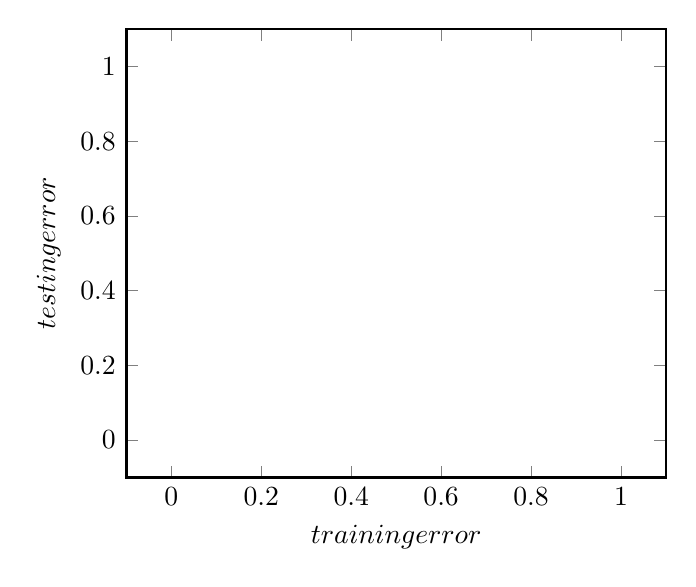
\begin{tikzpicture} %
		\begin{axis}[smooth,
		xlabel={$training error$}, %
		ylabel={$testing error$}, %
		legend pos = north east,%
		yticklabel style={/pgf/number format/.cd,fixed,precision=4},%
		line width=1pt%
		] %
		
		\end{axis} %
		\end{tikzpicture}
	}&
	\subfigure [2x] {
		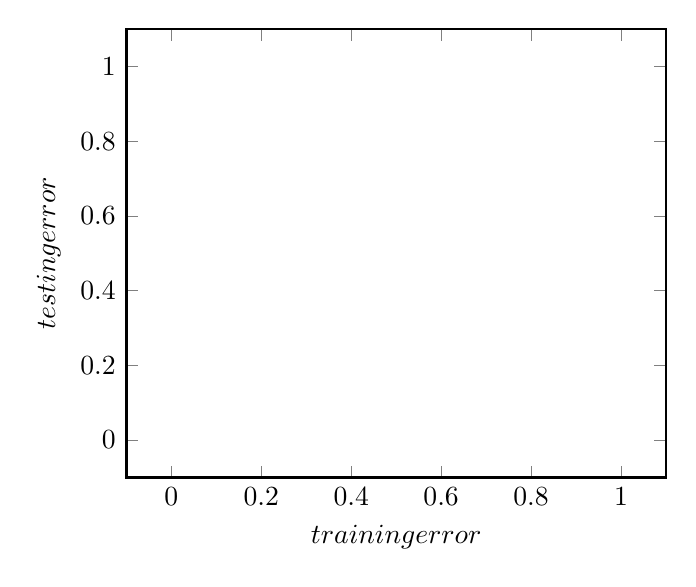
\begin{tikzpicture} %
		\begin{axis}[smooth,
		xlabel={$training error$}, %
		ylabel={$testing error$}, %
		legend pos = north east,%
		yticklabel style={/pgf/number format/.cd,fixed,precision=4},%
		line width=1pt%
		] %
		
		\end{axis} %
		\end{tikzpicture}
	}\\		
	\end{tabular}
	\caption {}
\end{figure}

%\addplot+[mark=ball] table[x expr=\coordindex , y={val_loss}] {\dnwtwoptinit};
%\addlegendentry{1xc};%							
\addplot+[
only marks,
mark=text, 
text mark={2}, 
text mark as node, 
text mark style=
{%
	font=\tiny,
	%circle,
	%inner sep=.02em,
	%fill=red!10!white,
	%draw=red,
},
] 
table[x expr=\coordindex , y={val_loss}, col sep=comma] {\dnwtwoptinit};
\addlegendentry{2xc};%	

\addplot+[
only marks,
mark=text, 
text mark={4}, 
text mark as node, 
text mark style=
{%
	font=\tiny,
	%circle,
	%inner sep=.02em,
	%fill=red!10!white,
	%draw=red,
},
] 
table[x expr=\coordindex , y={val_loss}, col sep=comma] {\dnwfooptinit};
\addlegendentry{4xc};%							
\addplot+[
only marks,
mark=text, 
text mark={6}, 
text mark as node, 
text mark style=
{%
	font=\tiny,
	%circle,
	%inner sep=.02em,
	%fill=red!10!white,
	%draw=red,
},
] 
table[x expr=\coordindex , y={val_loss}, col sep=comma] {\dnwsxoptinit};
\addlegendentry{6xc};%							

\addplot+[
only marks,
mark=text, 
text mark={8}, 
text mark as node, 
text mark style={%
	font=\tiny,
	%circle,
	%inner sep=.02em,
	%fill=red!10!white,
	%draw=red,
},
] 
table[x expr=\coordindex , y={val_loss}, col sep=comma] {\dnwegoptinit};
\addlegendentry{8xc};%							

\addplot+[
only marks,
mark=text, 
text mark={10}, 
text mark as node, 
text mark style={%
	font=\tiny,
	%circle,
	%inner sep=.02em,
	%fill=red!10!white,
	%draw=red,
},
] 
table[x expr=\coordindex , y={val_loss}, col sep=comma] {\dnwhnoptinit};
\addlegendentry{10xc};%

\addplot+[
only marks,
mark=text, 
text mark={12}, 
text mark as node, 
text mark style={%
	font=\tiny,
	%circle,
	%inner sep=.02em,
	%fill=red!10!white,
	%draw=red,
},
] 
table[x expr=\coordindex , y={val_loss}, col sep=comma] {\dnwhntwoptinit};
\addlegendentry{12xc};%							

\addplot+[
only marks,
mark=text, 
text mark={14}, 
text mark as node, 
text mark style={%
	font=\tiny,
	%circle,
	%inner sep=.02em,
	%fill=red!10!white,
	%draw=red,
},
] 
table[x expr=\coordindex , y={val_loss}, col sep=comma] {\dnwhnfooptinit};
\addlegendentry{14xc};%							

\addplot+[
only marks,
mark=text, 
text mark={16}, 
text mark as node, 
text mark style={%
	font=\tiny,
	%circle,
	%inner sep=.02em,
	%fill=red!10!white,
	%draw=red,
},
] 
table[x expr=\coordindex , y={val_loss}, col sep=comma] {\dnwhnsxoptinit};
\addlegendentry{16xc};%

\addplot+[
only marks,
mark=text, 
text mark={18}, 
text mark as node, 
text mark style={%
	font=\tiny,
	%circle,
	%inner sep=.02em,
	%fill=red!10!white,
	%draw=red,
},
] 

\fi